\documentclass[a4,paper,fleqn]{article}

\usepackage{layout}

\DeclareSIUnit\year{Jahr}
\newcommand{\wye}{
    \begin{tikzpicture}
        \draw ( 90:0) -- ( 90:0.2);
        \draw (210:0) -- (210:0.2);
        \draw (330:0) -- (330:0.2);
    \end{tikzpicture}
}

\title{Notizen EEV -- SW04}
\date{\today}
\author{Daniel Winz}

\begin{document}
\maketitle
\clearpage

\section{Erneuerbare Energie}

\subsection{Potential}
\begin{itemize}
    \item theoretisch: Angebot der Natur
    \item technisch: Erschliessungsmöglichkeiten
    \item realisierbar: wirtschaftliche Nutzung
\end{itemize}

\[ \text{Erntefaktor} = 
    \frac{\text{elelktrische Produktion eines Kraftwerks}}
         {\text{Energie zur Herstellung}} \]
\[ \text{Energetische Amortisationszeit} = 
    \frac{\text{Energie zur Herstellung}}
         {\text{elektrische Jahresproduktion}} \]

\section{Leistung einer Windanlage}
\begin{tabular}{@{}ll}
    $D$:        & Durchmesser des Rotors \\
    $\varrho$:  & Dichte der Luft \\
    $v$:        & Windgeschwindigkeit \\
    $\eta$:     & Wirkungsgrad \\
\end{tabular}
\\
Kinetische Energie eines Luftzylinders mit Masse $m$ und Geschwindigkeit $v$
\[ W_{kin} = \frac{1}{2} m v^2 \]
\[ m = v \cdot \varrho = A \cdot \ell \cdot \varrho \]
\[ A = frac{\pi \cdot D^2}{4} \]
\[ \ell = v cdot t \]
\[ \Rightarrow m = \frac{\pi D^2}{4} v \ell \varrho \]
\[ \Rightarrow W_{kin} = \frac{1}{8} \pi D^2 v^3 t \varrho \]
\[ \Rightarrow P_{Wind} = \frac{W_{kin}}{t} = \frac{1}{8} \pi D^2 v^3 \varrho \]

\section{Kernenergie CKW}
\begin{tabular}{@{}lr}
    Gössgen:                                & $\sim$  520 \si{\giga\watt\hour\per\year} \\
    Leibstadt:                              & $\sim$ 1020 \si{\giga\watt\hour\per\year} \\
    AKEB (AG für Kernenergiebeteiligungen): & $\sim$  750 \si{\giga\watt\hour\per\year} \\
    ENAG (Energiefinanzierungs AG):         & $\sim$  787 \si{\giga\watt\hour\per\year} \\
    Total:                                  & $\sim$ 3077 \si{\giga\watt\hour\per\year} \\
\end{tabular}

\section{Symmetrische Komponenten}
Ziel: Ein unsymmetrisches Drehstromsystem wird durch die Summe von 3 
symmetrischen Systemen dargestellt. 

\subsection{Drehstromoperator $a$}
\[ \boxed{\underline{a} = 1 \angle 120^\circ} \]
\begin{tikzpicture}
    \draw[-latex] (-2,0) -- (2,0) node[right] {Re};
    \draw[-latex] (0,-2) -- (0,2) node[above] {Im};
    \draw[-latex] (120:0) -- (120:1) node[below left] {$\underline{a}$};
\end{tikzpicture}
\[ a^2 = 1 \angle 240^\circ = 1 \angle -120^\circ \]
\[ a^2 = 1 \]
\[ a^4 = a \]
\[ 1 + a + a^2 = 0 \]
\[ a^2 - a = -j \sqrt{3} = \sqrt{3} \angle -90^\circ \]
\[ a - a^2 = j \sqrt{3} = \sqrt{3} \angle 90^\circ \]

\subsection{Mitsystem (Normalbetrieb)}
"'positive phase sequence"' \\
Index: 1 \\
\begin{tikzpicture}
    \draw[-latex] ( 60:0) -- ( 60:2) node[right] {$\underline{U}_{1L1} = \underline{U}_1$ (Bezug)};
    \draw[-latex] (180:0) -- (180:2) node[left]  {$\underline{U}_{1L3}$};
    \draw[-latex] (300:0) -- (300:2) node[right] {$\underline{U}_{1L2}$};
\end{tikzpicture}
\[ L_1: \underline{U}_{1L1} = \underline{U}_1 (Bezug) \]
\[ L_2: \underline{U}_{1L2} = \underline{a}^2 \underline{U}_1 \]
\[ L_3: \underline{U}_{1L3} = \underline{a}^1 \underline{U}_1 \]

\subsection{Gegensystem}
"'negative phase sequence"' \\
Index: 2 \\
\begin{tikzpicture}
    \draw[-latex] ( 60:0) -- ( 60:2) node[right] {$\underline{U}_{2L1} = \underline{U}_2$ (Bezug)};
    \draw[-latex] (180:0) -- (180:2) node[left]  {$\underline{U}_{2L2}$};
    \draw[-latex] (300:0) -- (300:2) node[right] {$\underline{U}_{2L3}$};
\end{tikzpicture}
\[ L_1: \underline{U}_{2L1} = \underline{U}_2 (Bezug) \]
\[ L_2: \underline{U}_{2L2} = \underline{a}^1 \underline{U}_1 \]
\[ L_3: \underline{U}_{2L3} = \underline{a}^2 \underline{U}_1 \]

\subsection{Nullsystem}
"'zero phase sequence"' \\
Index: 0 \\
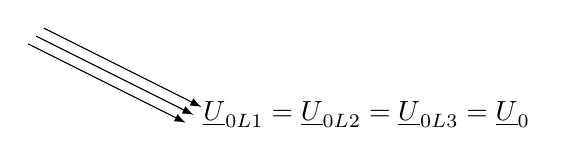
\begin{tikzpicture}
    \draw[-latex] (-0.0,-0.0) -- (2.0,-1.0);
    \draw[-latex] (-0.1,-0.1) -- (1.9,-1.1) node[right] {$\underline{U}_{0L1} = \underline{U}_{0L2} = \underline{U}_{0L3} = \underline{U}_0$};
    \draw[-latex] (-0.2,-0.2) -- (1.8,-1.2);
\end{tikzpicture}

\subsection{Bestimmung von $\underline{U}_1$, $\underline{U}_2$ und $\underline{U}_0$}
Bsp: Dreileiter Sternschaltung (ohne N) \\
\[
\left.
\begin{array}{@{}l}
\underline{U}_{1K} = \underline{U}_{1L1} + \underline{U}_{2L1} + \underline{U}_{0L1} \\\\
\underline{U}_{2K} = \underline{U}_{1L2} + \underline{U}_{2L2} + \underline{U}_{0L2} \\\\
\underline{U}_{3K} = \underline{U}_{1L3} + \underline{U}_{2L3} + \underline{U}_{0L3}
\end{array}
\right\rbrace \text{muss gelten}
\]

\[ \underline{U}_{1K} = \underline{U}_{1} + \underline{U}_{2} + \underline{U}_{0} \]
\[ \underline{U}_{2K} = \underline{a}^2 \underline{U}_{1} + \underline{a} \underline{U}_{2} + \underline{U}_{0} \]
\[ \underline{U}_{3K} = \underline{a} \underline{U}_{1} + \underline{a}^2 \underline{U}_{2} + \underline{U}_{0} \]
\rule{10cm}{0.5pt}
\[ \underline{U}_{1K} + \underline{U}_{2K} + \underline{U}_{3K} = 0 + 0 + 3 \underline{U}_{0} \]
\[ \boxed{\underline{U}_{0} = \frac{1}{3} \left(\underline{U}_{1K} + \underline{U}_{2K} + \underline{U}_{3K}\right)} \]
\subsection{Zusammenhang mit $\underline{U}_{K_N}$}
\[ \underline{U}_{1K} = \underline{U}_{1N} - \underline{U}_{KN} \]
\[ \underline{U}_{2K} = \underline{U}_{2N} - \underline{U}_{KN} \]
\[ \underline{U}_{3K} = \underline{U}_{3N} - \underline{U}_{KN} \]
\rule{10cm}{0.5pt}
\[ \underline{U}_{1K} + \underline{U}_{2K} + \underline{U}_{3K} = 0 - 3 \underline{U}_{KN} \]
\[ \Rightarrow \underline{U}_{0} = \frac{1}{3} (-3 \underline{U}_{KN}) \]
\[ \boxed{\underline{U}_{0} = -\underline{U}_{KN}} \]

\[ \underline{U}_{1K} = \underline{U}_{1} + \underline{U}_{2} + \underline{U}_{0} \]
\[ \underline{U}_{2K} = \underline{a}^3 \underline{U}_{1} + \underline{a}^2 \underline{U}_{2} + \underline{a} \underline{U}_{0} \]
\[ \underline{U}_{3K} = \underline{a}^3 \underline{U}_{1} + \underline{a}^4 \underline{U}_{2} + \underline{a}^2 \underline{U}_{0} \]
\rule{10cm}{0.5pt}
\[ \underline{U}_{1K} + \underline{a} \underline{U}_{2K} + \underline{a}^2 \underline{U}_{3K} = 3 \underline{U}_{1} + 0 + 0 \]
\[ \boxed{\underline{U}_{1} = \frac{1}{3} \left(\underline{U}_{1K} + \underline{a} \underline{U}_{2K} + \underline{a}^2 \underline{U}_{3K}\right)} \]

\subsection{Matrix}
\[
\left\lbrack
    \begin{array}{@{}l@{}}
        \underline{U}_{0} \\
        \underline{U}_{1} \\
        \underline{U}_{2} \\
    \end{array}
\right\rbrack
=
\frac{1}{3} \cdot
\underbrace{
    \left\lbrack
        \begin{array}{@{}ccc@{}}
            1 & 1               & 1               \\
            1 & \underline{a}   & \underline{a}^2 \\
            1 & \underline{a}^2 & \underline{a}   \\
        \end{array}
    \right\rbrack
}_{\lbrack t_1 \rbrack}
\cdot
\left\lbrack
    \begin{array}{@{}l@{}}
        \underline{U}_{1K} \\
        \underline{U}_{2K} \\
        \underline{U}_{3K} \\
    \end{array}
\right\rbrack
\]
\[ \lbrack t_1 \rbrack \Rightarrow \text{Taschenrechner} \]

\subsection{Sternschaltung unsymmetrisch mit N (Vierleitersystem)}
\[
\left\lbrack
    \begin{array}{@{}l@{}}
        \underline{I}_{0} \\
        \underline{I}_{1} \\
        \underline{I}_{2} \\
    \end{array}
\right\rbrack
=
\frac{1}{3} \cdot
\lbrack t_1 \rbrack
\cdot
\left\lbrack
    \begin{array}{@{}l@{}}
        \underline{I}_{L1} \\
        \underline{I}_{L2} \\
        \underline{I}_{L3} \\
    \end{array}
\right\rbrack
\]
\[ \underline{I}_{L1} + \underline{I}_{L2} + \underline{I}_{L3} = \underline{I}_{N} \]
\[ \underline{I}_{L1} = \frac{1}{3} \underbrace{(\underline{I}_{L1} + \underline{I}_{L2} + \underline{I}_{L3})}_{I_N} \]
\[ \boxed{\underline{I}_{N} = 3 \cdot \underline{I}_{0}} \]

\subsection{Rücktransformation}
\[
\left\lbrack
    \begin{array}{@{}l@{}}
        \underline{U}_{1K} \\
        \underline{U}_{2K} \\
        \underline{U}_{3K} \\
    \end{array}
\right\rbrack
=
\frac{1}{3} \cdot
\lbrack t_1 \rbrack^{-1}
\cdot
\left\lbrack
    \begin{array}{@{}l@{}}
        \underline{U}_{0} \\
        \underline{U}_{1} \\
        \underline{U}_{2} \\
    \end{array}
\right\rbrack
\]

\end{document}
